\subsection{Telecommunication}


\begin{frame}{Telecommunication}{Line-Of-Sight}
  \begin{columns}[T]
    \begin{column}{.5\textwidth}
      \begin{block}{}
        \begin{itemize}
          \item {At high frequencies (above 30MHz) the ability to see the antenna roughly corresponds to the ability of receive the radio signal.}
          \item {Radio Horizon: Furthest possible point of propagation.}
          \item {OBS: Altitude with respect to the WGS84 datum.}
        \end{itemize}
      \end{block}
    \end{column}
    \begin{column}{.5\textwidth}
      \begin{figure}
        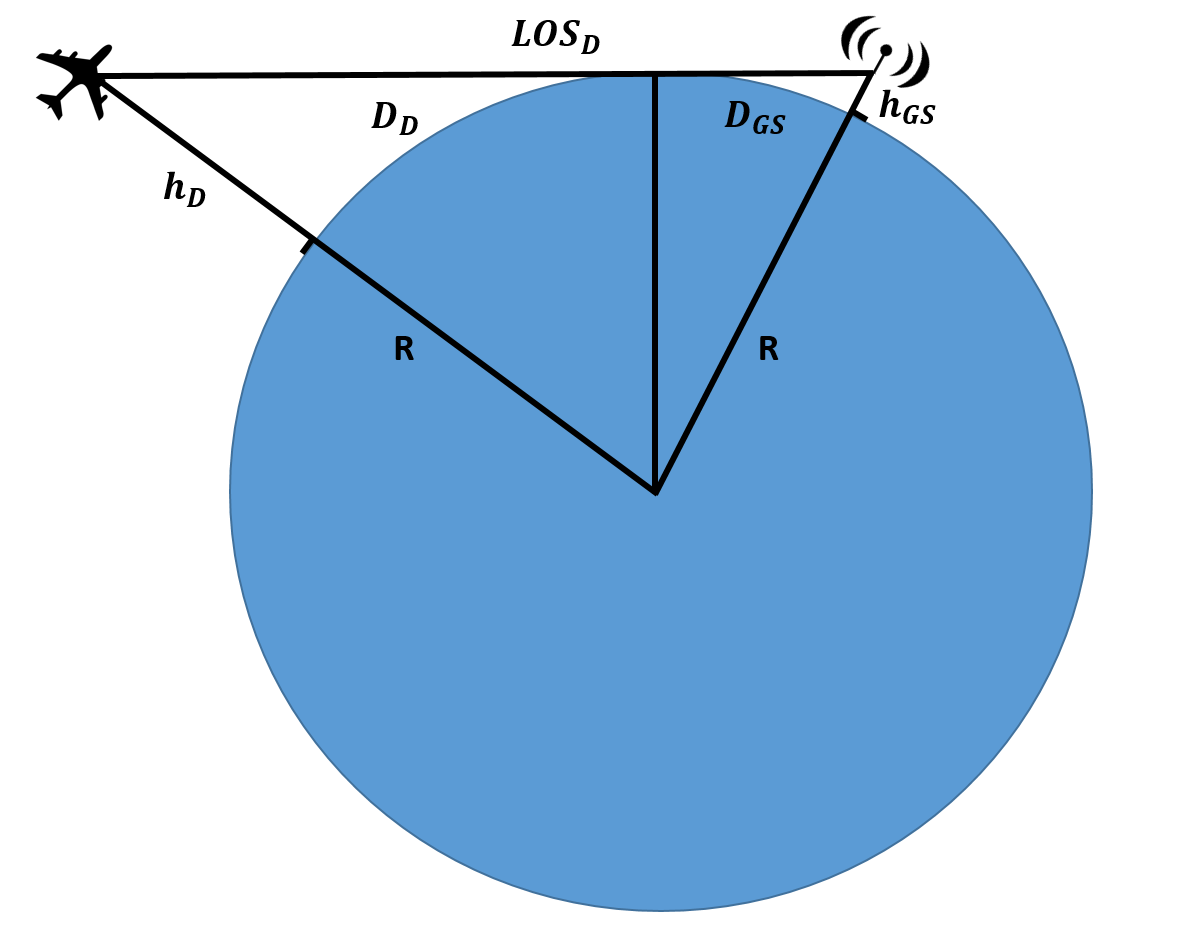
\includegraphics[scale=0.25]{figures/LOS.png}
      \end{figure}
    \end{column}
  \end{columns}

    \begin{align*}      
        LOS_d[km]  \approx {3.57\cdot (\sqrt{h_D[m]} + \sqrt{h_{GS}[m]}} )
    \end{align*}

\end{frame}


\begin{frame}{Telecommunication}{Link Budget}
  \begin{columns}[T]
    \begin{column}{.5\textwidth}
      \begin{block}{}
        \begin{itemize}
          \item {At high frequencies (above 30MHz) the ability to see the antenna roughly corresponds to the ability of receive the radio signal.}
          \item {Radio Horizon: Furthest possible point of propagation.}
          \item {OBS: Altitude with respect to the WGS84 datum.}
        \end{itemize}
      \end{block}
    \end{column}
    \begin{column}{.5\textwidth}
      \begin{figure}
        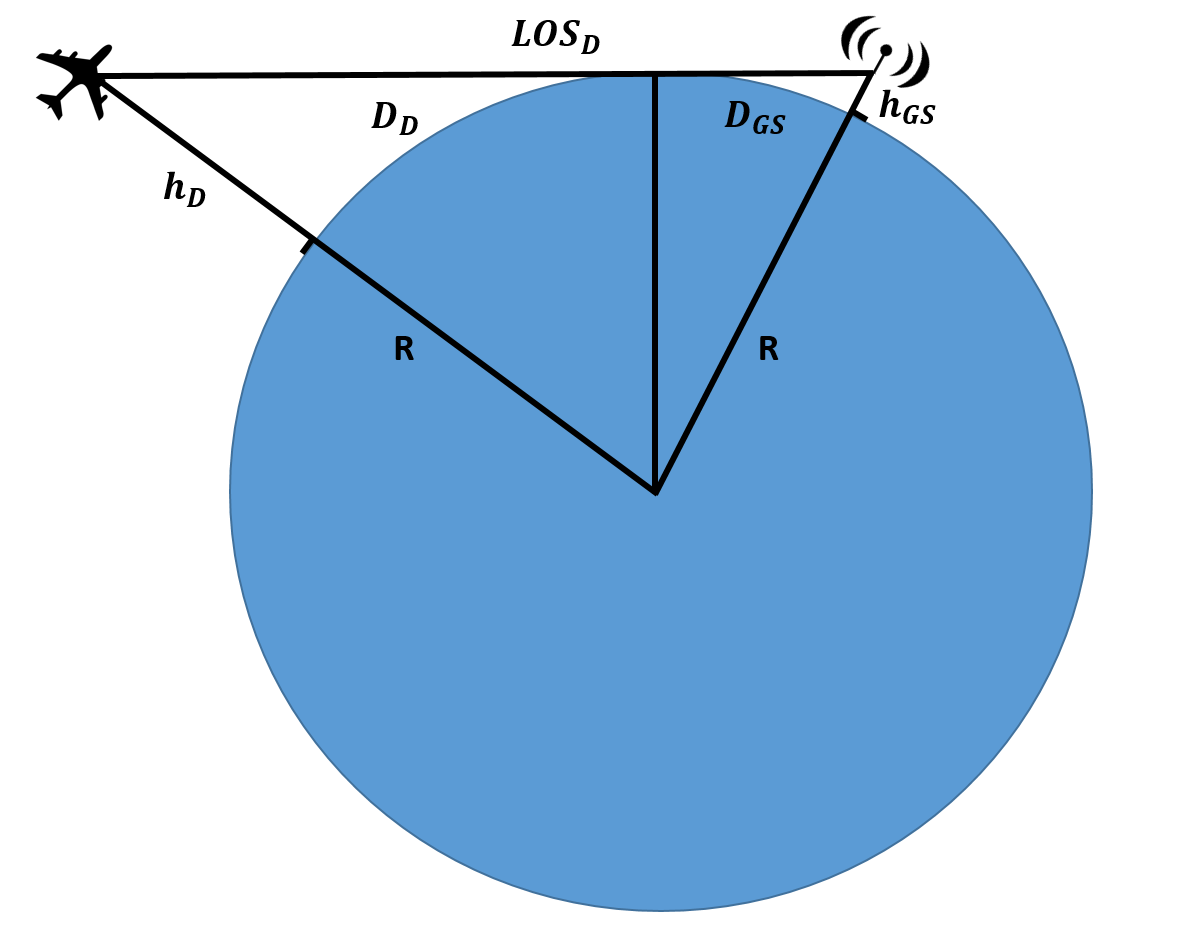
\includegraphics[scale=0.25]{figures/LOS.png}
      \end{figure}
    \end{column}
  \end{columns}

    \begin{align*}      
        LOS_d[km]  \approx {3.57\cdot (\sqrt{h_D[m]} + \sqrt{h_{GS}[m]}} )
    \end{align*}

\end{frame}

\begin{frame}{Telecommunication}{Fresnel Zones}
  \begin{columns}[T]
    \begin{column}{.5\textwidth}
      \begin{block}{}
        \begin{itemize}
          \item {At high frequencies (above 30MHz) the ability to see the antenna roughly corresponds to the ability of receive the radio signal.}
          \item {Radio Horizon: Furthest possible point of propagation.}
          \item {OBS: Altitude with respect to the WGS84 datum.}
        \end{itemize}
      \end{block}
    \end{column}
    \begin{column}{.5\textwidth}
      \begin{figure}
        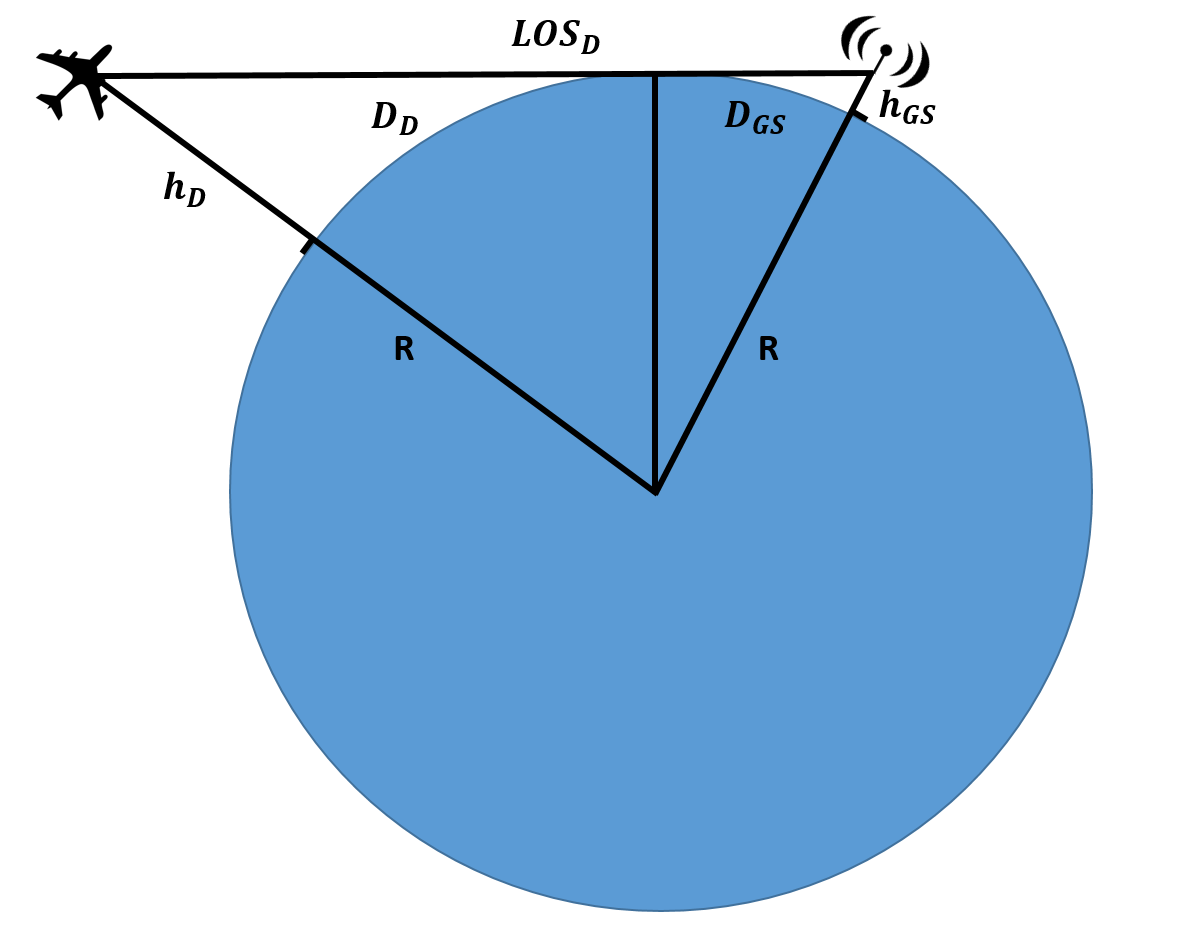
\includegraphics[scale=0.25]{figures/LOS.png}
      \end{figure}
    \end{column}
  \end{columns}

    \begin{align*}      
        LOS_d[km]  \approx {3.57\cdot (\sqrt{h_D[m]} + \sqrt{h_{GS}[m]}} )
    \end{align*}

\end{frame}